\section{Introduction}
\label{sec:introduction}

Techniques for dynamic dependency analysis have been fruitful, with applications ranging from information-flow security~\cite{sabelfeld03} and optimisation~\cite{kildall73} to debugging and program comprehension~\cite{weiser81,delucia96}. There are, however, few methods suitable for fine-grained analysis of richly structured outputs, such as data visualisations and multidimensional arrays. Dataflow analyses \cite{reps95} tend to focus on analysing variables rather than parts of structured values. Where-provenance~\cite{buneman01} and related data provenance techniques are fine-grained, but specific to relational query languages. Taint tracking \cite{newsome05} is also fine-grained, but works forwards from input to output. For many applications, it would be useful to be able to focus on a particular part of a structured output, and have an analysis isolate the input data pertinent only to that substructure.

This is a need that increasingly arises outside of traditional programming. Journalists and data scientists use programs to compute charts and other visual summaries from data, charts which must be interpreted by colleagues, policy makers and lay readers alike. Interpreting a chart correctly means understanding what the components of the visualisation actually \emph{represent}, i.e.~the mapping between data and visual elements. But this is a hard task, requiring time and expertise, even with access to the data and source code used to create the visualisation. In practice it is easy for innocent (but devastating) mistakes such as transposing two columns of data to go unnoticed~\cite{miller06}.

\subsection{Motivation}
\label{sec:introduction:motivation}
Before outlining our contributions, we consider two motivating examples from the domain of data visualization. Our techniques are not limited to this area. They are simply cases of programs that transform structured input data (a data table) to structured output data (components of a chart). The first challenge is linking outputs to the inputs that were used to produce them.

\paragraph{Linking structured outputs to structured inputs}
Interpreting a chart would be much easier if the user was able to explore the relationship between the computed components of a chart and the underlying data, revealing the relevant relationships on a need-to-know basis. As illustrated in \figref{introduction:data-linking} below, selecting a particular bar in the bar chart should highlight the data relevant to a selected bar in the table showing the source data (the figure only shows subset of the full table):

\begin{figure}[H]
   \begin{subfigure}[b]{0.99\textwidth}
      \centering
      {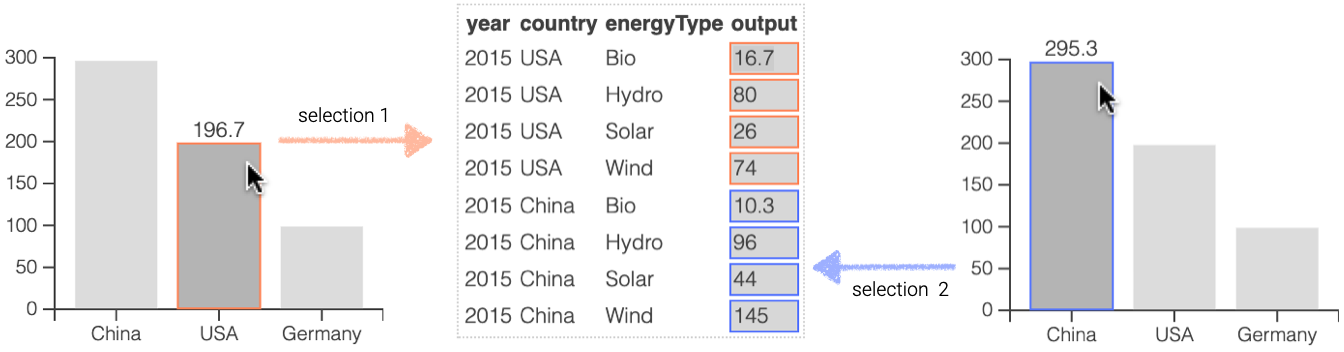
\includegraphics[scale=0.36]{fig/example/data-linking-merged.png}}
   \end{subfigure}\\
   \begin{subfigure}{0.65\textwidth}
      \small
      \lstinputlisting[language=Fluid]{fluid/bar-chart.fld.mod}
   \end{subfigure}
   \caption{Fine-grained linking of outputs to inputs, focusing on data from USA (left) and China (right). }
   \todo{Maybe ``selection 1'' and ''selection 2'' instead of ``Backwards'' above}
   \label{fig:introduction:data-linking}
\end{figure}

Visualisation designers sometimes create ``data-linked'' artefacts like these by hand, such as Nadieh Bremer's award-winning visualisation of population density growth in Asian cities~\cite{bremer15}, but this requires significant programming effort. Libraries such as Altair \cite{vanderPlas18} alleviate some of this work, but they require specifying data transformations using a limited set of combinators provided by (and understood by) the library.

We frame the challenge as a program analysis problem. We want to be able to focus on a particular chart element and determine the inputs that contribute to it. This is a matter of selecting a part of the structured output and performing some kind of backwards analysis that identifies the relevant data. The advantage of this approach is that data linking comes ``for free'', and the data scientist is able to code their analyses as pure functions using an expressive language as done in \figref{introduction:data-linking}.

\paragraph{Linking structured outputs to other structured outputs}
Program analysis going backwards, from output charts to input data, supports one kind of information visualizations, but there is more to be done. Visualizations often present distinct but related aspects of data in multiple charts. In this situation the user should be able to focus on (select) a visual element in one chart or other structured output and automatically see elements of a different chart which were computed using related inputs. For example in \figref{introduction:vis-linking} below, selecting a bar on the left should automatically highlight all the related visual elements on the right. This is a well-recognised use case called \emph{brushing and linking}~\cite{becker87}.

\begin{figure}[H]
  \begin{subfigure}[b]{0.99\textwidth}
     \centering
     {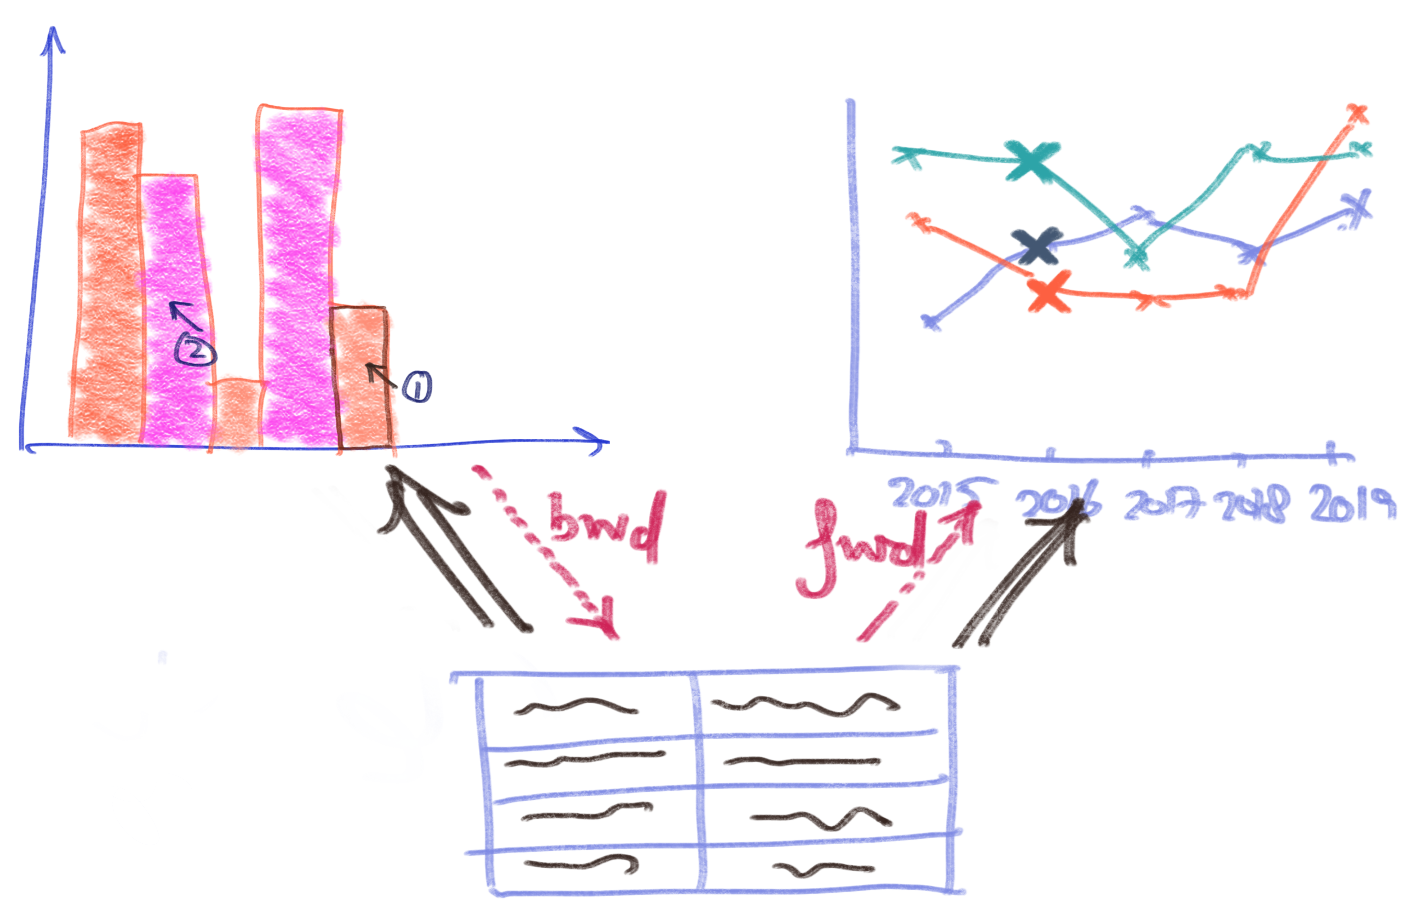
\includegraphics[scale=0.58]{fig/example/vis-linking.png}}
  \end{subfigure}\\[2mm]
  \begin{subfigure}{0.8\textwidth}
     \small
     \lstinputlisting[language=Fluid]{fluid/line-chart.fld.mod}
  \end{subfigure}
 \caption{Linking visualisations via common data dependencies}
 \label{fig:introduction:vis-linking}
 \todo{Need mouse cursor and selected value ($196.7$) on LHS. Maybe ``User selection'' and ``computed selection''}
\end{figure}

Geospatial applications like GeoDa~\cite{anselin06} and charting libraries like Plotly support brushing and linking, but they tend to be baked into specific applications, or require programmer effort and therefore must be anticipated in advance by the chart designer. Moreover these applications and libraries provide no direct way for the reader to see the common data which explains why elements are related.

We can again frame this as a program analysis problem. It is a matter of selecting a part of the structured output and performing a backwards analysis to identify the required inputs, as before, but then performing a further forwards analysis to identify dependent parts of the other output. A combination of backward and forward analysis would provide a language-based foundation for brushing and linking, allowing it to be used automatically with ordinary programmatic data transformations such as those showin in \figref{introduction:vis-linking} above.
%but also ``data-transparent'', able to provide a concise view of the data that underpin a given relationship.

\subsection{Contributions}

To solve these problems, we need a dependency analysis which supports focusing on substructures of rich outputs, and moreover one which can be used bidirectionally, with appropriate round-tripping properties. Recent program slicing techniques \cite{perera12a,perera13a,ricciotti17} allow the user to focus on the output by ``erasing'' parts deemed to be irrelevant; the erased parts, called \emph{holes}, are propagated backwards by a backwards analysis which identifies parts of the program and input which are no longer needed. Although these approaches enjoy useful round-tripping properties characterised by Galois connections, they only allow focusing on \emph{prefixes} of a structured output, rather than arbitrary substructures.

In this paper, we present new language-based data provenance technique for linking structured outputs, such as visualisations, to structured inputs, and to each other, in a fine-grained way. Our work advances the state of the art \todo{phrase differently and revisit in light of \secref{toolkit}} of program analysis in three ways:

\begin{itemize}
\item Our bidirectional dependency analysis makes it possible to select any part of a resulting data structure. This makes it possible to determine what parts of inputs and code contribute to a part of a value that has been produced.
\item The backward and forward analaysis that we define can be composed in a number of ways to perform a range of useful data analyses. In addition to combining backwards and forwards analyses, as discussed above, we can achieve other functionality by inverting the selection before performing the analysis.
\item We implement and formalize a rich surface language with familiar functional programming features including piecewise definitions, pattern matching, list notation and list comprehensions. Doing so in a way that supports bidirectional program analysis requires careful consideration.
\end{itemize}

\noindent The rest of the paper is structured as follows. We introduce a core calculus in \secref{core-language}. In \secref{data-dependencies} we define a bidirectional data dependency analysis and prove that it forms a Galois connection. \secref{toolkit} describes how this analysis and its de Morgan dual are used in our PureScript implementation to support the kind of linking scenarios motivated above, and compares our approach to related work. \secref{surface-language} presents the surface language, and shows it desugars into the core language via another Galois connection. \secref{conclusion} summarises and discusses opportunities for future work.

%In this paper, we present new language-based data provenance techniques for linking structured outputs, such as visualisations, to structured inputs, and to each other, in a fine-grained way. Our specific contributions are as follows:

% \begin{itemize}
%   \item[--] a new bidirectional dependency analysis for a core calculus with lists, vectors and records, and a proof that the analysis is a Galois connection (\secref{core-language});
%   \item[--] applications of the core analysis to enrich visualisations with interactions which allow a user to explore their relationship to data and to each other, and a comparison with \emph{Galois slicing}, a program slicing framework with similar round-tripping properties (\secref{toolkit});
%   \item[--] a richer surface language called \OurLanguage with familiar functional programming features, including piecewise definitions, pattern matching, list notation and list comprehensions, and an extension of our analysis to the desugaring (\secref{surface-language});
%   \item[--] an implementation of Fluid in PureScript, a discussion of strengths and weaknesses of the approach, and opportunities for future work (\secref{evaluation}).
%\end{itemize}
